% Copyright 2004 by Till Tantau <tantau@users.sourceforge.net>.
%
% In principle, this file can be redistributed and/or modified under
% the terms of the GNU Public License, version 2.
%
% However, this file is supposed to be a template to be modified
% for your own needs. For this reason, if you use this file as a
% template and not specifically distribute it as part of a another
% package/program, I grant the extra permission to freely copy and
% modify this file as you see fit and even to delete this copyright
% notice.

\documentclass{beamer}
\usepackage[utf8]{inputenc}
\usepackage{amsmath}
\usepackage{amsthm}
\usepackage{amssymb}
\usepackage{xcolor}
\usepackage{enumerate}
\usepackage[overload]{empheq}
\usepackage{filecontents}
\usepackage{graphics}

\usepackage{graphicx}

\usetheme{Singapore}
\setbeamertemplate{navigation symbols}{}
\setbeamertemplate{footline}[frame number]{}

\title{ACO for SSCFLP}

\author{Dorian Dumez \& Samuel Buchet}

\date{may 30 2017}

\AtBeginSection[]
{
  \begin{frame}<beamer>{Sommaire}
    \tableofcontents[currentsection]
  \end{frame}
}
%\AtBeginSubsection[]
%{
%  \begin{frame}<beamer>{Sommaire}
%    \tableofcontents[currentsection,currentsubsection]
%  \end{frame}
%}

% Let's get started
\begin{document}

\begin{frame}
  \titlepage
\end{frame}

\begin{frame}{Table Of Content}
  \tableofcontents
  % You might wish to add the option [pausesections]
\end{frame}

\section{Single Source Capacitated Facility Location Problem}

\begin{frame}{Presentation of the problem}

    \begin{figure}
        \centering
        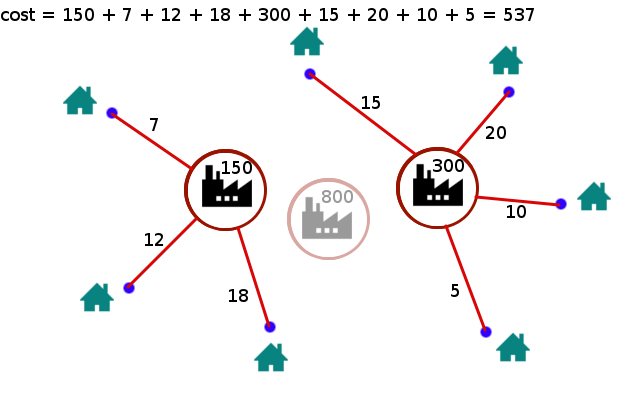
\includegraphics[scale=0.3]{schema}
    \end{figure}

    \begin{itemize}
        \item NP-hard combinatorial optimization problem
        \item m places to (eventually) open facilities
        \item n customers to be connected to the facilities
        \item each facility has an opening cost and a demand
        \item each customer has a connection cost and a capacity
        \item goal: minimize the cost
    \end{itemize}

\end{frame}

\begin{frame}{Linear program}
    \begin{figure}
    \centering
    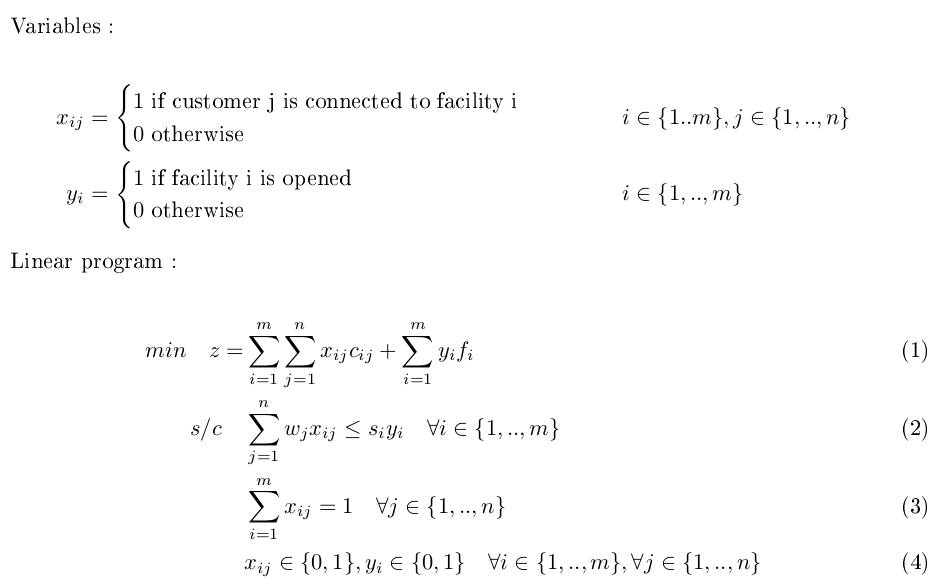
\includegraphics[scale=0.32]{model}
\end{figure}
\end{frame}

\section{Ant Colony Optimization}

\begin{frame}{Global shape}
Branch only on association customer/facility :
\begin{itemize}
\item
pheromone and heuristic are in matrices $\mathbb{R}^{n \times m}$, one value for each association
\item
heuristic information is $1/ \text{association cost}$, it doesn't take in account the opening cost
\item
to construct a solution we take each customer and associate them with a lean wheel over the facility with enough remaining capacity
\end{itemize}
\end{frame}

\begin{frame}{Update pheromone method}
3 designs implemented :
\begin{itemize}
\item
ACS : all ant are equal \\
$\Delta \tau_{ij} = \sum \limits_{bs \in T} \Delta \tau_{ij}^{bs}$
\item
EAS : only best one drop off \\
$\Delta \tau_{ij} = \sum \limits_{i = 1}^{\text{nbElite}} \Delta \tau_{ij}^{bs\left[i\right]}$
\item
rank base : best one leave more \\
$\Delta \tau_{ij} = \sum \limits_{i = 1}^{\text{nbAnt}} \Delta \rho^i \tau_{ij}^{bs\left[ i \right] }$, $\rho \in \left[ 0 ; 1 \right] $
\end{itemize}
Where $\Delta \tau_{ij}^{bs} = \frac{\delta_{bs.association}(i,j)}{bs.val}$
\end{frame}

\section{Local search}

\begin{frame}{Principle}
    \begin{itemize}
        \item definition of a neighborhood
        \item the neighborhood is explored
        \item hopefully a better solution is found
        \item the process is repeated until the solution cannot be improved anymore
    \end{itemize}
\end{frame}

\begin{frame}{Local Search for FLP}
    \begin{figure}
        \centering
        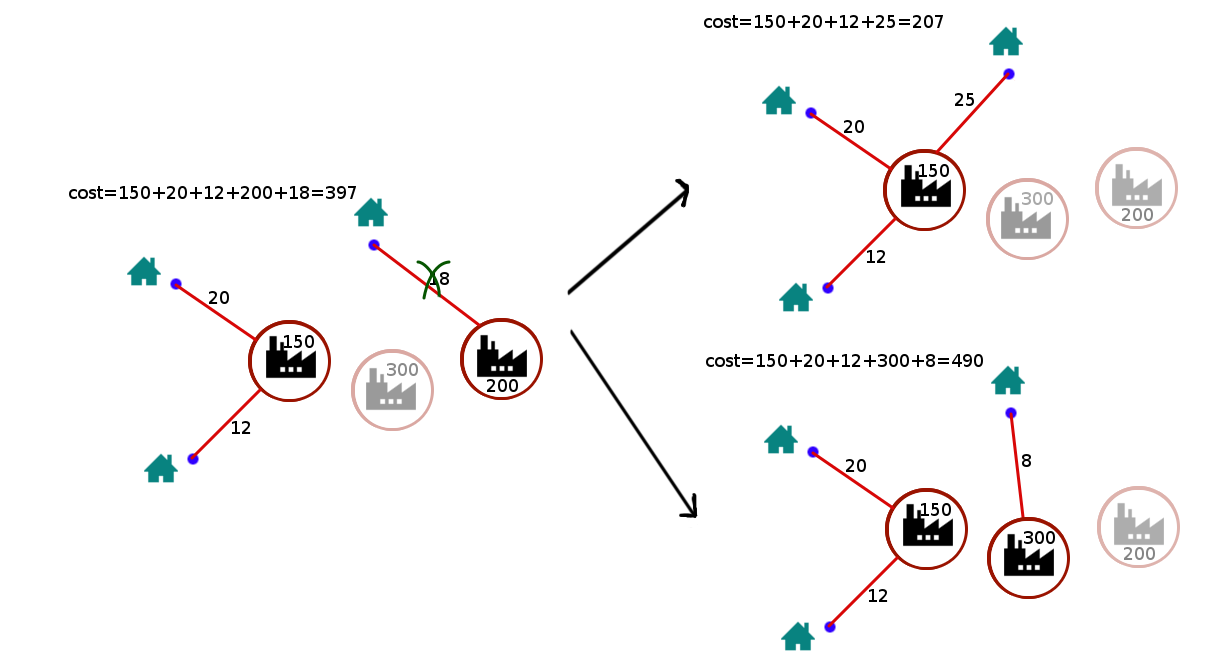
\includegraphics[scale=0.27]{schemalstot}
        \caption{ one move = connect a customer to another facility}
    \end{figure}
\end{frame}

\section{Experiments}

\begin{frame}{Using irace}
\begin{itemize}
\item
Parameter setting have been done by irace
\item
We use a set of 71 instances of different size :
\begin{itemize}
\item
56 were used as training set
\item
21 were used as testing set
\end{itemize}
\item
At the end of the run irace think he can get better results with more time
\item<2->
Demonstration with output parameter
\end{itemize}
\end{frame}

\begin{frame}{Further improvement}
\begin{itemize}
\item
Perform a longer irace run
\item
Branch over the facility opening too :
\begin{itemize}
\item
modify pheromone and heuristic
\item
adapt the construction algorithm
\end{itemize}
\item
Try other local search, like VND
\item
Try other pheromone update schema

\end{itemize}
\end{frame}

\section*{Conclusion}

\begin{frame}{Conclusion}
\begin{itemize}
\item
Like that it's pretty bad, but it's complicated problem
\item
With an improved version we should be able to speed up exacts algorithms
\end{itemize}
\end{frame}

\section{References}

\begin{frame}{References}

\begin{itemize}

    \item Icons made by \href{http://www.freepik.com}{Freepik} from \href{http://www.flaticon.com}{www.flaticon.com} is licensed by \href{http://creativecommons.org/licenses/by/3.0/}{Creative Commons BY 3.0}

    \item Icons made by \href{http://www.flaticon.com/authors/icomoon}{Icomoon} from \href{http://www.flaticon.com}{www.flaticon.com} is licensed by \href{http://creativecommons.org/licenses/by/3.0/}{Creative Commons BY 3.0}

\end{itemize}

\end{frame}

\end{document}
